\documentclass[preview]{standalone}
\usepackage{tikz}
\usetikzlibrary{arrows}

\begin{document}
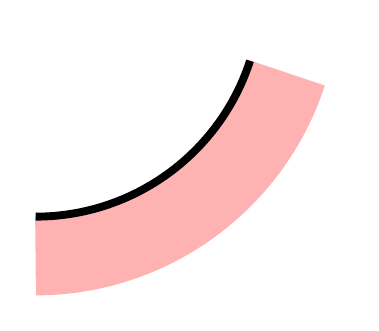
\begin{tikzpicture}[scale=1,
rotate = 180, 
stretch/.style={color=red!30, line width=1cm},
solid/.style={line width=1mm}]

\def\pressure{80}
\def\hx{4}	
\def\hy{1}  % change only with line width of stretch
\def\yshift{1.5}	% Shift zwischenden principles
\pgfmathsetmacro{\hyh}{.5*\hy}
\pgfmathsetmacro{\hxh}{\hx/2}


\path[clip] (0.1,-.9)rectangle++(-4.1,-3.5);

\pgfmathsetmacro{\alp}{90*\pressure/100}
\def\pi{3.1416}
\pgfmathsetmacro{\r}{\hx/\alp*180/\pi*.9}
% Bended
\draw[stretch] (0,-\yshift)arc(90:90+\alp:\r+\hyh);
\draw[solid] (0,-\hyh-\yshift)arc(90:90+\alp:\r);



\end{tikzpicture}
\end{document}